\documentclass[12pt]{article}

\usepackage[paper=letterpaper,margin=2.5cm]{geometry} % Set Margins

%% Math and math fonts
\usepackage{amsmath, amsthm, amssymb, amsfonts}
\usepackage{bbm} % for \mathbbm{1}

% Color
\usepackage{color, xcolor}

% Misc
\usepackage{environ}  % \collect@body in asmmath
\usepackage{graphicx} % \includegraphics options
\usepackage{mdframed} % text boxes
\usepackage{indentfirst} % Indent first paragraph after section header
\usepackage[shortlabels]{enumitem} % Control enumerate items with [(a)]
\usepackage{comment} % Comments
\usepackage{fancyhdr} % Headers and footers

% Tables
\usepackage{array}

% Sub-figures and figure placement
\usepackage{caption}
\usepackage{subcaption}
\usepackage{float} 

% Graphing
\usepackage{pgfplots}
\pgfplotsset{compat=1.17}
\usepackage{tikz}

% Title Placement
\usepackage{titling}
\setlength{\droptitle}{-6em}

% Images 
\usepackage{pgfplots}


% %%%% Theme %%%% % Colors from https://yaleidentity.yale.edu/web
% \definecolor{YaleBlue1}{HTML}{00356b}
% \definecolor{YaleBlue2}{HTML}{286dc0}
% \definecolor{YaleBlue3}{HTML}{63aaff}
% \definecolor{YaleGray1}{HTML}{222222}
% \definecolor{YaleGray2}{HTML}{4a4a4a}
% \definecolor{YaleGray3}{HTML}{978d85}
% \definecolor{YaleGray4}{HTML}{dddddd}
% \definecolor{YaleWhite}{HTML}{f9f9f9}
% \definecolor{YaleGreen}{HTML}{5f712d}
% \definecolor{YaleOrange}{HTML}{bd5319}

%set indent to 
\setlength{\parindent}{0pt}

%for headers 
\pagestyle{fancy}

\lhead{Creel}
\chead{Review}
\rhead{Nature as Capital}

\title{Section 6 -- Midterm Review}
\author{Andie Creel}
\date{March 27th, 2023}

% Hyper refs
\usepackage{hyperref}
\hypersetup{
    colorlinks=true,
    linkcolor=blue,
    urlcolor  = blue,
    filecolor=magenta,      
    urlcolor=blue,
    citecolor = blue,
    anchorcolor = blue
}

% % Citation management
% \usepackage{natbib}
% \bibliographystyle{agsm}
% \setcitestyle{authordate,open={(},close={)}}

\begin{document}
\maketitle

\section{Marginal Value of Another "Unit"}

\subsection{Lagrangian case}
In the Lagrangian case, we have a budget constraint. Therefore, we may be interested in the marginal value of another unit of budget. 
\begin{align}
    \mathcal{L} = U(x,y) + \lambda(B - wx - vy) \label{lagrang}
\end{align}
To find the marginal value of another unit of budget, we can take the derivative of the Lagrangian \ref{lagrang} (which measures value) with respect to the budget $B$,

\begin{align}
    \frac{\partial \mathcal{L}}{\partial B} = \lambda.
\end{align}

Therefore $\lambda$ is the marginal value of another unit of budget (\textit{aka.} the marginal utility of money) in the Lagrangian case. 

\subsection{Hamiltonian Case}
In the Hamiltonian case, we are interested in a stock that grows following $\dot s$. Our current value Hamiltonian is

\begin{align}
    H_t &= W(s_t, h(s_t)) + \lambda_t \dot s_t \label{hamil}\\ 
    &= dividends + capital \ gains
\end{align}


Recognize that $\lambda_t$ is the marginal value of another unit of stock in the Hamiltonian case. \\

In problem set three, you were asked what the marginal value of a mammoth is in the first time period. You should have recognized that this was asking for the shadow price in time period one, \textit{i.e.,} the marginal value of another unit of stock (which is the definition of a price). The first optimality condition gave you a solution for the shadow price as a function of harvest, which is what we expected you to use to calculate the shadow price.\\

To solve for an explicit equation for the shadow price $\lambda$ refer to section \ref{euler_section} on the Euler equation.

\section{Implicit Functions review}
Implicit versus explicit 
$U(x,y)$ versus $x^{\beta}y^{1-\beta}$\\
$U(C)$ versus $\frac{C^{1 - \eta}}{1 - \eta}$\\
$G(s)$ versus $sr(1 - \frac{s}{K})$\\

Q: If I was a company and produced widgets using produced capital natural capital, how would you write an implicit function to represent production? \\
A: $F(N, P)$ where $N$ is natural capital and $P$ is produced capital. 

\section{Logistic Growth and Graphs}
$$ \dot x = \frac{\partial x}{\partial t} = rx(1 - \frac{x}{K})$$

Where will $\dot x = 0$? There are 2 roots, so there are 2 spots it will equal zero. It's already factored, so set each part equal to zero. 

$$ 1 - x/K = 0 \implies x_{ss} = K$$
$$ rx = 0 \implies x_{ss} = 0$$

When $x > 0$ but $ x < K$ we know the growth rate is positive. When $x > K$, the growth rate is negative. Therefore we know when $x_{ss} = K$ is a stable point, b/c if $x$ is perturbed, it will return to $K$. 

\begin{figure}[h]
    \centering
    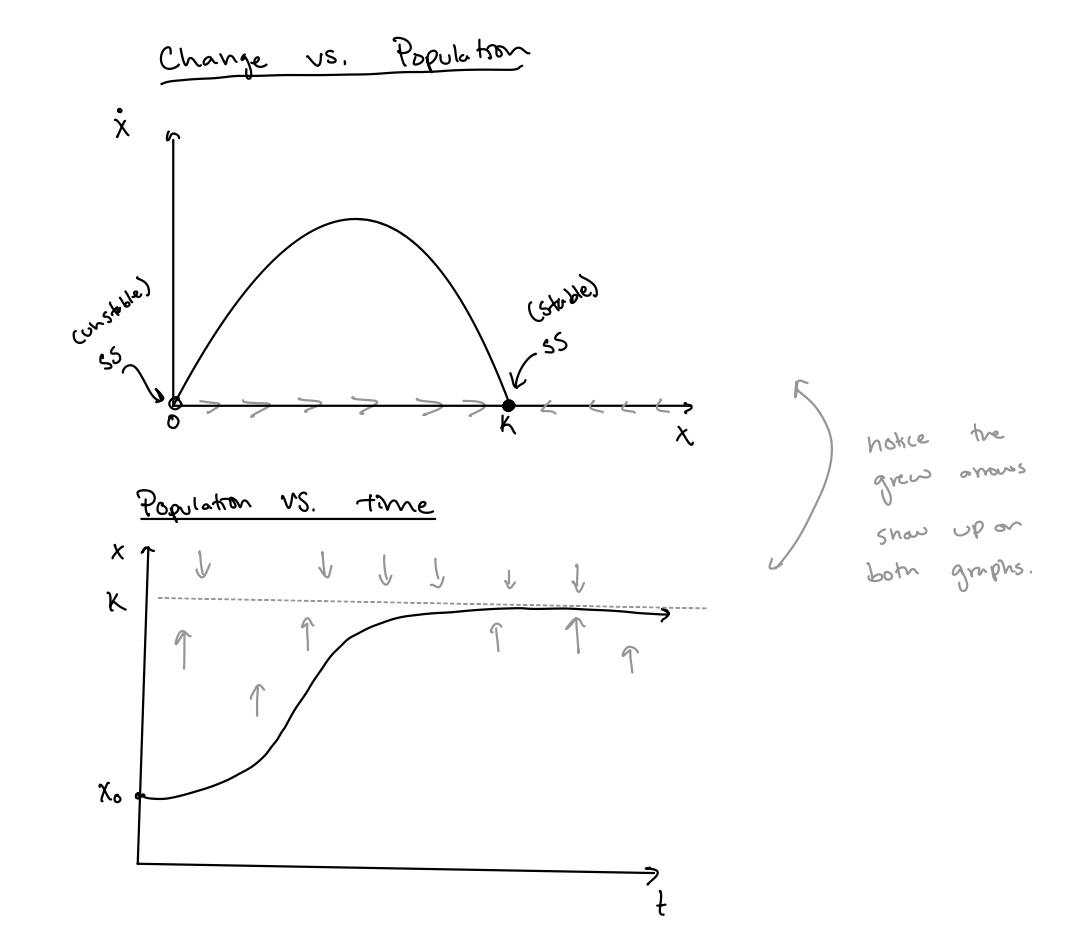
\includegraphics[width=0.6\textwidth]{logistic_growth.png}
    \caption{"grew" should say grey}
    \label{fig:my_label}
\end{figure}

\section{Logistic Growth with Harvest}
$$ \dot x =rx(1 - \frac{x}{K}) - h $$ 

Where will $\dot x = 0$? When $h = rx(1 - \frac{x}{K})$. Consider the case where our harvest program is $h = \frac{x}{4}$. Could then set  $rx(1 - \frac{x}{K}) = \frac{x}{4}$ and solve for $x_{ss}$. \\

When $h < rx(1 - \frac{x}{K})$, the growth rate $\dot x$ is positive. When $h > rx(1 - \frac{x}{K})$, the growth rate $\dot x$ is negative.

\begin{figure}[h]
    \centering
    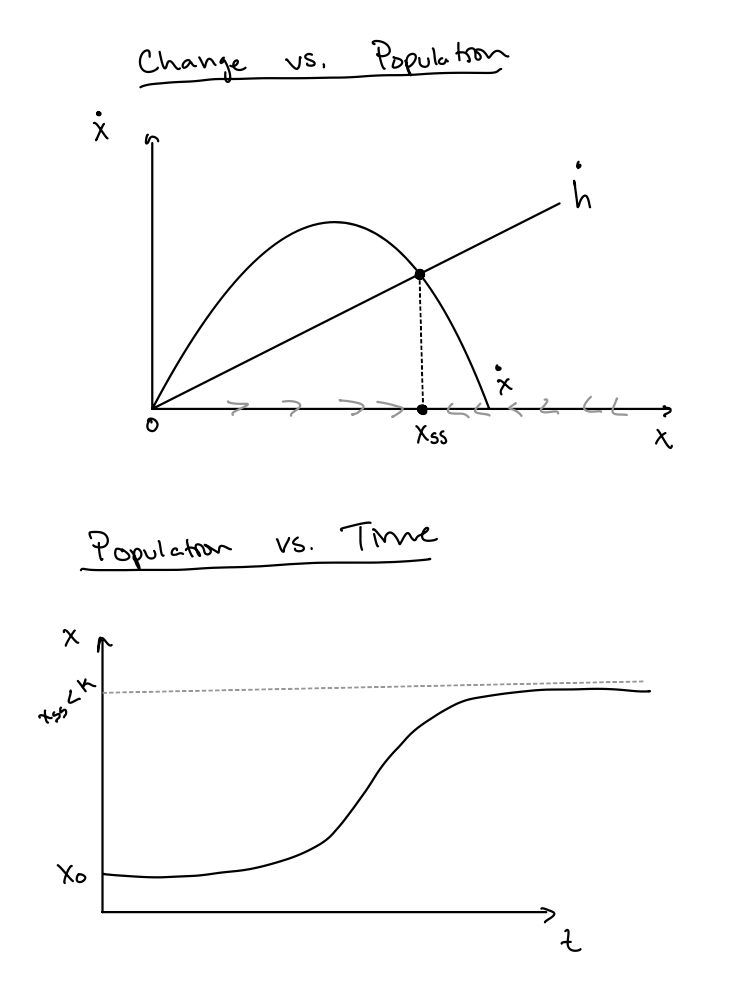
\includegraphics[width=0.6\textwidth]{harvest.png}
    \caption{The steady-state level of population is less than its carrying capacity when there is a harvest}
    % \label{fig:my_label}
\end{figure}

\textbf{Note:} I would focus on reviewing logistic growth, then be conceptually familiar with a few other types of ecological growth. Review the week two class notes on ecological models. 


\section{Euler Equation to get Shadow Price \label{euler_section}}

\subsection{Easy Version \label{easy_vers}} 
Start with the Current Value Hamiltonian 
\begin{align}
    \delta V = H = W(s, h) + \lambda \dot s. \label{CVH_1}
\end{align}

Solve for the value, $V$, 
$$V = \frac{W(s, h) + \lambda \dot s}{\delta}.$$
Recall the shadow price is defined as the marginal value of an additional unit of stock. Find $\frac{\partial V}{\partial s}$ and solve for $\lambda$ to get the Euler equation which gives us the shadow price,
\begin{align}
    \lambda = \frac{\partial V}{\partial s} = \frac{W_s + \dot \lambda}{\delta - \dot s_s}. \label{euler}
 \end{align}   
\ref{euler} is the Euler equation and tells us what our shadow price $\lambda$ is equal to. 

\subsection{Not so hard but slightly longer version}
We can derive the current value Hamiltonian from the intertemporal welfare function and then get the Euler equation.\\

The present value of a stock where the "present" time period is 0 can be found using our intertemporal welfare function,
\begin{align}
    V(s(t)) = \int_0^\infty W(s(\tau), x(s(\tau)) \exp(-\delta\tau)d\tau. \label{inter_welf}
\end{align}

For small changes in time, we can take the derivative of the LHS and RHS. This exercise will eventually reveal the CVH in equation \ref{CVH_1}. \\

Left Hand Side of \ref{inter_welf} (uses the chain rule, also recall marginal value = capital price (i.e., $\frac{\partial V}{\partial s} = \lambda(s)$) and that the derivative with respect to time uses dot notation (i.e., $\frac{\partial s}{\partial t} = \dot s$)): 

\begin{align}
    \frac{\partial V(s(t))}{\partial t} = \frac{\partial V}{\partial s} \frac{\partial s}{\partial t} &= \lambda(s) \dot s\\
    &= capital \ gains
    \label{LHS}
\end{align}


Right Hand Side of \ref{inter_welf} (Leibniz rule for the derivative of integral, don't stress if you don't follow this calculus step):

\begin{align}
    \frac{\partial \int_t^\infty W(s(\tau), x(s(\tau)) \exp(-\delta(\tau-t))d\tau}{\partial t}= \delta V(s(t)) - W(s, x(s)) 
    \label{RHS}
\end{align}


Setting \ref{LHS} = \ref{RHS} and doing a tiny bit of algebra, we get 


\begin{align}
    \delta V(s(t)) = W(s, x(s)) + \lambda(s) \dot s 
    \label{hamil}
\end{align}

which is the same as our current value Hamiltonian from equation \ref{CVH_1}! \\

You can then follow the same steps in section  \ref{easy_vers} to get the Euler Equation for the capital/shadow price. 

\section{Calculating Wealth}
Not doing p*q except if you're finding a lower bound. 


\section{Review from in Class}

\subsection{Present vs Current Value Hamiltonian}
\textbf{PVH:}  \\
Discrete value: $H_p = W(S, h) \beta^t + \lambda (G(s) -h)$\\
Continuous value: $H_p = W(S, h) e^{-\delta t} + \lambda (G(s) -h)$\\
\textit{The units} of a PVH will always be in 2023 dollars (or whatever time period zero is). \textit{The units} of $\lambda$ are in present-year dollars. \\


\textbf{CVH:}\\
Continuous time: $ H_c = W(S, h) + \lambda e^{\delta t} (G(S) - h)$\\
which can be rewritten as $H_c = W(S,h) + \mu_t (G(S) - h).$\\
\textit{The unit} of the CVH will be in year $t$ dollars. \textit{The units} of $\mu$ are in current-year dollars. \\

\textbf{Going between the two:}\\
$\mu_t = \lambda e^{\delta t}$\\
$e^{\delta t} * $PVH =  CVH\\
The only reason we use the CVH more often is that the CVH has easier algebra. \\

\textbf{Recall that the shadow price comes from the Lagrangian}
\begin{align}
    \mathcal{L} = U(x,y) + \lambda (B - vx -  wy)\\
    \frac{\partial \mathcal{L}}{\partial B} = \lambda
\end{align}

Note that how a stock grows can also be a constraint:
\begin{align}
    \mathcal{L} = \sum_t U(S_t, h_t) \beta^t + \beta \lambda_{t+1}(S_t + G(S_t, h_t) - S_{t+1})\\
\end{align}

\subsection{Steady States}
Consider the mammoth problem: 
\begin{align}
    M_{t+1} = M_t + G(M_t) - h_t\\
    \frac{\Delta M}{\Delta t} = M_{t+1} - M_t = G(M_t) - h_t \label{SS}
\end{align}

In steady state, $\frac{\Delta M}{\Delta t} = 0$, because the population isn't changing anymore. \\
$\frac{\Delta M}{\Delta t} = 0$ \& \ref{SS} $ \implies h_{10} = G(h_{10})$. \\
You could then solve for $h_{10}$ to get the harvest you can take from period 10 until forever. \\
The get the annuity value of this harvest level you can find 
$$annuity \ value = \frac{U(h_{10}) \beta^{10}}{\delta}$$


\subsection{Changes in wealth and changes in welfare}
\begin{align}
    V(S_t) = \int U(S(\tau))e^{\delta (\tau - t)} \partial \tau \\
    s.t. \ \dot S\\
    \frac{\partial V(S_t)}{\partial t} = U_S - \delta V \label{Vt_1}\\
    \frac{\partial V}{\partial t} = \frac{ \partial V}{\partial S}\frac{\partial S}{\partial t} \label{Vt_2}\\
    \delta V = U_s + \frac{\partial V}{\partial S} \dot S \label{CVH}
\end{align}
Notice that \ref{CVH} is a current value Hamiltonian. \ref{Vt_1} and \ref{Vt_2} imply \ref{CVH}. This is how we derive the CVH. 


\begin{align}
    W =\sum pS\\
    \frac{\partial W}{\partial t} = \sum p \dot S
\end{align}

\subsection{Discounting}
\textbf{Ramsey Rule:} Start with constant elasticity of utility 
$$U = \frac{C^{1 - \eta} - 1}{1 - \eta}$$
$$\dot S = F(s) - C$$
$$\int_0^\infty U(C) e^{-\delta t}$$

$$r = \delta + \eta F'(S)$$

There are two ways to discount, $\delta$ and $\eta$. $\delta$ is how we discount between generations. $\eta$ is how we discount the growth of wealth. $F'(S)$ is a growth rate. Typically we think future generations are going to be wealthier. Ramsey argues that $\delta$ should be set equal to zero, but that $\eta$ should be non-zero because we can borrow from the rich of tomorrow in order to benefit the poor of today.\\

A high discount rate would be that we need to borrow from tomorrow to redistribute wealth to today. A low discount rate would be that we favor future generations. 

\subsection{"Combine mathematical expressions"}
If you have two equations equal to the same thing (say 0), then "combining mathematical expressions" means setting those equations equal to one another. 

\end{document}